%%==================================================
%% chapter03.tex for SJTU Bachelor Thesis
%% version: 0.5.2
%% Encoding: UTF-8
%%==================================================

% \bibliographystyle{sjtu2} %[此处用于每章都生产参考文献]



\chapter{系统架构}
\label{chap:archi}

\section{系统环境}

本文章所对应实现的主要目的有两个,第一点是从学术大数据中提取学术会议之间的相关关系,并将其以可视化的形式表现出来.第二点则是利用学术大数据以及其中学术会议之间的相关关系,为在阅读查找学术论文时,想要寻找主题相近的文章的人提供帮助的一个推荐算法.

数据来源为微软公司截止至2016年2月所收集的论文的各种信息,包括题目,作者,会议,摘要等等.选作为数据源的论文为筛选出的包含论文数量最多的前一千个会议.论文总数为1514255篇,用于训练词向量的文本总大小为1.2GB.

整个项目基本上由Python语言编写而成,训练词向量的环境为Ubuntu 14.04 LTS, Python 2.7, Tensorflow 1.0版本,通过GeForce GTX 1080显卡GPU进行训练.

从词聚类到会议向量生成一直到推荐系统应用以及可视化数据的生成也是通过Python进行.主要原因是系统主要处理对象为大量格式化数据,而又夹杂了包括神经网络在内的一系列工程方面的实现,Python作为一个新兴的面向对象的脚本语言,生态环境良好.既拥有以Numpy,Pandas为首的一系列支持数据处理的优秀的包,也同时是几个主要的神经网络框架Theano\footnote{\url{http://deeplearning.net/software/theano/}},Tensorflow\footnote{\url{https://www.tensorflow.org/}}等选择的接口平台,还可以很方便的搭建工程,管理系统,可以说是用来搭建本系统的最好选择.并且笔者对Python的特性较为了解,能够很迅速地利用Python中带有的各种语法糖来编写简短有效的代码段,易于开发调试.



\subsection{Tensorflow}

Tensorflow是由Google公司旗下Google Brain的研究小组开发的一种利用数据流图来进行数值计算的一个开源的软件包.从它的名字中可以看出,在这里的数据流是以张量的形式来参与计算的.所谓的张量,简单来说也就是有固定"形状"的多维数组.严格的来说,Tensorflow并不是一个仅仅能用于训练神经网络的框架,但Tensorflow拥有设计优秀使用简便的C++/Python接口,配合上它固有的数据流图的使用特性,会让搭建个性化的神经网络变得十分简单,而对多核CPU以及显卡等辅助计算工具的良好支持又使得它在提升效率上能给予我们很多帮助,所以Tensorflow目前也成为搭建训练神经网络的首选框架之一.

在Tensorflow之中,搭建好的神经网络被称为一个"图".而图是由节点和边构成的.Tensorflow中的图里的节点就是一个一个的张量,也就是多维数组.这些多维数组通常是在搭建图的时候就决定好了其尺寸和具体数值,可以是固定的值常量constant,也可以是在训练中能够改变的值变量Variable,但也有特殊的情况.在我们的输入层和最后输出层计算损失函数时就需要用到训练数据,这部分在模型搭建时是不知道的,但我们可以提前知道它在网络中的位置和后续的操作,我们利用占位符placeholder来代表这一类的节点.


而节点与节点之间的连接关系称为边,在Tensorflow中,每一条边都代表了一个张量操作.可以是简单的与标量的加减乘除四则运算,也可以是复杂的矩阵运算,还可以在张量上应用激活函数,算结果与标签的交叉熵,取各种统计量等做法.采用Tensorflow的优势就在于我们不用自己去实现复杂的矩阵操作,而是可以将整个张量视作整体,来在比较宏观的角度来思考我们所搭建的网络结构,这样能够很大程度上提升网络搭建的效率,而不是自己仔细地去写一个个复杂的循环.在图\ref{fig:tf}中有搭建简单网络的示意图,可以在从图中大致了解网络的组成和训练的流程.

以下是一个简单的通过Tensorflow搭建神经网络训练识别手写字符(MINST)的示例代码

\begin{python}
import tensorflow as tf
# 训练变量定义
x = tf.placeholder("float", [None, 784]) 
y_ = tf.placeholder("float", [None,10])
W = tf.Variable(tf.zeros([784,10]))
b = tf.Variable(tf.zeros([10]))

# 网络搭建
y = tf.nn.softmax(tf.matmul(x,W) + b)
cross_entropy = -tf.reduce_sum(y_*tf.log(y))
train_step = tf.train.GradientDescentOptimizer(0.01).minimize(cross_entropy)
init = tf.initialize_all_variables()

# 开始训练
with tf.Session() as sess:
	sess.run(init)
	for i in range(1000):
	  batch_xs, batch_ys = mnist.train.next_batch(100)
	  sess.run(train_step, feed_dict={x: batch_xs, y_: batch_ys})

\end{python}

可以看到,我们搭建的网络是由一层简单的全连接层组成,输入为784(28*28)而输出为10,激活函数采用Softmax,损失函数采用的是经常被用于多标签分类问题的交叉熵,采用梯度下降算法进行训练.一个网络的搭建仅仅需要几行代码,并且通过读取代码中的函数名称等,基本上就能掌握网络的整体结构,训练也可以很方便的通过调用一个run函数来实现,实在是搭建以及训练神经网络的利器.

\begin{figure}
  \centering
  \subfigure[Tensorflow节点示意]{
    \label{fig:tf} %% label for first subfigure
    \includegraphics[height=0.4\textwidth]{chap3/tf.png}}
  \hspace{1in}
  \subfigure[Gephi图示意]{
    \label{fig:gephi} %% label for second subfigure
    \includegraphics[height=0.4\textwidth]{chap3/gephi.png}}
  \caption[工具框架示例]{工具框架示例}
  \label{fig:tf_gephi}
\end{figure}

\subsection{Gephi}

Gephi是一款开源免费的跨平台网络分析软件.主要应用于对网络和各种复杂系统之中的各类大数据集的动态,分层交互可视化以及探测.常见用途可以是用来对科研项目中实验数据进行分析,或是对统计信息进行分析研究,例如新闻分析,微博,推特分析等等.

Gephi是用Java编程语言,基于NetBeans平台开发的,通过JVM可以实现跨平台.其可视化引擎是完全基于OpenGL的API,并且由于其完全开源,使用者完全可以通过应用OpenGL的标准API来自己定制所需要的插件,编写符合自己要求的新功能或者对旧的显示选项进行修改等等,总而言之是一款非常好用且灵活的大数据可视化软件.

在Gephi中,我们通过定义节点和边以及它们之间的关系来定义一幅图.节点之间可以通过有向边或者是无向边来相互连接,而节点和边本身又可以携带很多信息,例如节点编号,节点标签,边的编号,标签,种类,权重等等.我们可以很方便的自己添加各种信息,来在图中体现各种各样的数据集合.同时,我们定义好的图可以也就可以通过二元组$(V,E)$来表示,其中节点和边的信息可以作为csv文件导入导出,使用非常简便,也方便Gephi程序本身与后端处理数据的Python代码对接.从图\ref{fig:gephi}中可以看到用Gephi作为可视化工具画出来的图.非常美观大方,又可以清晰的看到数据点之间的关系.




\section{系统模块}

整个系统分为两大部分,会议关系可视化以及基于会议关系的论文推荐系统.其中两个系统的前端是相通的,进行处理的基本思路是相同的,或者可以说会议关系可视化是对基于会议关系的论文推荐系统的一个补充,二者在功能上相辅相成,基本原理也是一样的.

前端则是从最开始的词向量生成一直到会议向量生成.可以将整个前端理解成一个独立的系统,这个系统以学术论文数据库为输入,最终能够生成有良好性质的会议向量以及各个文章向量来辅助我们进行数据分析.

\subsection{词向量生成}

根据在前文\ref{subsec:word2vec}中所提到的方法,我们采用Word2Vec的方法来实现从论文数据到词向量的转化.首先我们来观察我们所拥有的数据情况.在微软公司提供的数据库中,我们可以根据一篇论文的编号,得到其标题,作者,发表的会议以及其摘要,下载地址等信息.那么我们应该采用哪些数据,又应该放弃哪些数据来进行词向量生成呢?

这个时候我们就应该把目光从当前的词向量放得更远一些,想清楚我们为什么需要这些词向量,我们最后会怎么应用这些词向量,怎么样才能使得生成的这些词向量更符合我们之后所需要的应用呢?这样一想我们就豁然开朗了.我们的根本目的是生成能够很好比较相似性,甚至于一些更复杂的相关关系的会议向量.而这么做的好处是我们可以为寻找关注于某一类论文的用户提供更好的推荐服务.那么,显然我们应该让词向量能够更好的反应这篇文章所关注的重点,所归属的学术分类.更具体地说,是需要找到一个词,在整个语料库,整个学术论文数据库中,所代表含义的综合体.通过这个综合的意义,来组成代表这个词的词向量.

所以在经过分析之后,我们考虑的是将每篇论文的摘要和标题作为训练数据来训练词向量.首先论文正文数据量过于庞大,并且比较杂乱,里面会夹杂一些没有用,或者无法体现出文章特点的词语,数据等等,稀释了训练的成果.而其余的数据并没有办法直接地拿来放到神经网络中去训练一个词向量.所以我们就得到了以所有文章的摘要组成的训练语料.

词向量的训练通过在Tensorflow上实现Word2Vec算法来执行.值得一提的是,由于在搭载NVidia GeForce GTX 1080显卡的机器上进行训练,所以在训练时采用了GPU模式,将训练速度提高到了原来的20到30倍,这也要归功于Tensorflow前后端分离的架构,能让在显卡GPU上的部署变得非常方便.

网络搭建部分的代码如下示例

\begin{python}
# From word2vec.py
def build_graph(self):
    opts = self._options

    (words, counts, words_per_epoch, self._epoch, self._words, examples, labels) = word2vec.skipgram(
            filename=opts.train_data,
            batch_size=opts.batch_size,
            window_size=opts.window_size,
            min_count=opts.min_count,
            subsample=opts.subsample
            )
    (opts.vocab_words, opts.vocab_counts,
     opts.words_per_epoch) = self._session.run([words, counts, words_per_epoch])
    opts.vocab_size = len(opts.vocab_words)


    self._examples = examples
    self._labels = labels
    self._id2word = opts.vocab_words
    for i, w in enumerate(self._id2word):
        self._word2id[w] = i
    true_logits, sampled_logits = self.forward(examples, labels)
    loss = self.nce_loss(true_logits, sampled_logits)
    self._loss = loss
    self.optimize(loss)

    # Properly initialize all variables.
    tf.global_variables_initializer().run()
\end{python}

由于Word2Vec本身的结构较为简单,仅仅是拥有一个中间层的神经网络,所以在Tensorflow上进行网络的搭建本身是非常简单的事情.不过要考虑到一个训练批次的问题.所谓的训练批次,就是在利用损失函数更新网络参数时,如果每次只计算一组数据带来的损失,计算效率过低不说,还会大大地降低运行的并行度,让利用GPU变得毫无意义.所以我们每次更新网络参数的时候会综合多组数据计算出的损失,这多组数据一起就叫一个训练批次.现在流行的神经网络的实现,通常都采用以批次为单位来训练的方法.

那么下面的问题,就变成我们应该选择同时将多少组数据当做一个批次,进行并行的训练了.选择的批次过小可能会导致训练数据之间相互影响抵消,导致结果不能很好的收敛,而训练批次过大会让算法收敛的很快,但很有可能会收敛到一个并不是很好的局部最优点,而几乎不可能摆脱出来.理由也很好解释.在批次过小时,在神经网络的训练过程中,选择合适的训练批次大小也是一个非常有意义的话题,它们都从属于超参数学习的研究范围,在这里就不赘述了.


以下是Word2Vec训练词向量的部分的代码.

\begin{python}
# From word2vec.py
def main(_):
    opts = Options()
    mConfig = tf.ConfigProto(allow_soft_placement=True)
    mConfig.gpu_options.allocator_type = 'BFC'
    mConfig.gpu_options.per_process_gpu_memory_fraction=0.8
    with tf.Graph().as_default() as graph, tf.Session(config=mConfig) as session:
        with tf.device("/gpu:0"):
            model = Word2Vec(opts, session)

        for epoch in xrange(opts.epochs_to_train):
            model.train()                              
            model.save_vec(FLAGS.vector_path, epoch) 

        # Perform a final save.
        model.saver.save(session,
                os.path.join(opts.save_path, "model.ckpt"),
                global_step=model.global_step)      
    
\end{python}

可以看到还是非常简单的步骤,设定好一些参数之后就可以进行训练和结果的保存.可以稍微一提的是,这里我自己实现了一个支持多线程的Skip-gram模型数据读取转换工具,是为了支持在自己的CPU机器上进行高速的并行训练.不过因为最终训练的场所是GPU机器,这里就没有用上,也是一种遗憾吧.这里就稍微贴上一部分代码可以参考一下.

\begin{python}
#!/usr/bin/python
import threading
class SkipgramReader:
    """Self-Customed Skipgram Reader"""
    def __init__(self, batch_size, window_size, file_path, word2id):
        self.window_size = window_size
        self.file_path = file_path
        self.batch_size = batch_size
        self._word2id = word2id
        self.EOF = True
        self.batch_lock = threading.Lock()
        self.init_lock = threading.Lock()
        self.initial()

    def get_next_batch(self):
        self.batch_lock.acquire()
        next_batch = []
        for i in xrange(self.batch_size):
            status, res = self.get_next_pair()
            if not status:
                next_batch += [[0,0] for _ in xrange(self.batch_size)]
                break
            next_batch.append(res)           
        self.batch_lock.release()
        return self.EOF, next_batch

    def initial(self):
        self.init_lock.acquire()
        if self.EOF:
            self.fd = open(self.file_path, 'r')
            self.cur_char = ' '
            self.word_queue = list()
            self.cur_pos, self.cur_off = 0, 0            
            for i in xrange(2*self.window_size+1):
                self.insert_next_word()
            self.EOF = False
        self.init_lock.release() 
   
   ...
\end{python}

\subsection{词聚类与文章向量生成}

在获得了由Word2Vec利用了学术论文数据库中的摘要而训练处词向量之后,我们接下来考虑的就是如何利用这一组词向量来构成文章向量.那么和在生成词向量之前同样的,我们就必须在这么做之前考虑应该怎么做,为什么要这么做的问题.首先为什么要生成文章向量呢?那是因为考虑到我们的目的,是为了最后的学术会议的相关性研究以及以此为基础的推荐算法的实现,所以我们在之前的章节\ref{sec:recomm}中介绍的算法里面考虑过后,发现基于内容的推荐算法是比较适合我们这整个系统的实现的.

第一点就是基于协同过滤的算法的评价矩阵在这个场景下是很难取得的,学术搜索引擎的使用者比起电商网站和各种文章网站的使用者来说,目的性更为强烈.而基于内容的推荐算法由于只需要考虑目标本身的数据,加上我们已经借由Word2Vec模型获得了整个数据集的词向量,以此来进行文章的向量化特征提取就是一件水到渠成的事情了.

那么我们怎么做到这件事情呢?在\ref{sec:content-based}中我们也曾经研究过这一点,借由之前的结论我们可以发现,做词聚类后的文章向量生成应该是一个比较合理的方案.首先,学术论文中专业名词的比例会远远高于普通论文,特别是在需要在很短的篇幅中让人清楚地大体认识到整个文章内容的摘要里面,就更是如此了.那么我们经由摘要训练出的词向量,聚类之后的结果显然是会很具有代表性的.其次,词聚类还能避免很多词向量之间的影响导致信息的流失,这一点之前也有提出过了,就不再赘述.

至于对聚类算法的选择,这里我们在\ref{sec:cluster}中已经讨论过了各个不同种类的聚类算法之间的差异和优劣比较.作为比较大数据集合,并且数据分布在高维空间中,有很好的区分度的时候,我们就会采取最为直接的划分式聚类算法.这里采用的就是普通的\textbf{K-Means}算法,由于算法过于简单,就不在这里再过多描述了.

在得到了词聚类之后,我们就采用\textbf{tf-idf}的方法来进行文章向量的构建,作为变量的单位当然是聚类.以下是供参考的部分代码片段.

\begin{python}
# From doc2vec.py
from sklearn.preprocessing import scale


def load_clusters(path):    
    word2cluster = dict()
    file_list = os.listdir(path)
    for each in file_list:
        if each in ['.', '..']: continue
        with open(os.path.join(path, each), 'r') as f:
            for line in f:
                try:
                    cluster_index, word = line.strip().split(',')
                    word2cluster[word] = int(cluster_index)
                except ValueError as detail:
                    print("ValueEroro in loading clusters: ", detail)
                    pass
    return word2cluster
word2cluster = load_clusters(path_cluster)
multiple_space = re.compile(r'\s+')
illegal_char = re.compile(r'[^A-Za-z]')

# Clean illegal characters and redundant space
def wash_doc(raw):
    # Wash dirty data    
    clean = multiple_space.sub(" ", illegal_char.sub(' ', raw))
    return clean

def gen_doc_vec(doc):
    global word2cluster
    new_doc_vec = [0.0 for _ in xrange(opt.vec_dim)]
    for word in doc:
        new_doc_vec[word2cluster.get(word, 0)] += 100
    new_doc_vec_scaled = scale(new_doc_vec).tolist()
    return new_doc_vec_scaled

def write_doc_vec(doc_vecs, path):
    assert len(doc_vecs) > 0
    delim = " "
    with open(path, 'w') as f:
        for vec in doc_vecs:
            f.write(delim.join(map(str, vec)))
            f.write('\n')

\end{python}


\subsection{会议向量生成与相关性分析}

在得到了文章向量之后,我们要做的最后一步就是生成对应的会议向量了.当然到了最后一步我们仍然不能盲目地尝试,还是要思考我们的目的以及为了达成目的而选择的手段.得到了以词聚类频率为分量的文章向量,那么可以说我们的系统已经完成了一大半.因为这个时候的文章向量,配合上词聚类本身的意义,是非常容易解读的.什么样子的单词在这篇文章的摘要里出现,很直接地就决定了这篇文章背后所蕴含的学术成果的方向.很明显地是,这个时候我们自然大可以像一些文章网站所采用的简单的推荐系统那样,直接利用文章向量之间的相似度,来做基于内容的推荐系统.但那样做会碰到两个问题.

第一,跳过会议向量的生成,直接进行推荐,是无法达成我们想要研究学术会议之间的相关性的目的的.通过分散的学术论文,我们很难很直观地去描述它们所对应的那个学术会议究竟是怎么样的存在.或者说,很难用一种机器的方式,去直接通过文章向量描述一个学术会议.

第二,会议中的文章和文章所投搞发表的会议之间所关注的主题,我们不应该看做是一个单方向的蕴含关系.并不仅仅是由发表的文章决定了某个学术会议所关注的主题.同样的,研究者们在投稿的时候,当然很自然地会去考虑他们的文章应该往哪一个学术会议去投稿发表.学术会议本身在召开前,邀请投稿的时候,也都会给出自身所需稿件的研究主题的范围.这二者是一个相互影响的关系,而仅仅采用文章向量去描述一个会议,就会损失掉这部分的信息.

那么我们的选择就是,将一个学术会议中的所有文章向量都集合起来,综合地表示一个会议.之后在考虑反过来利用这个会议向量,来去做文章之间的推荐.那么怎么去生成这个会议向量呢?这时候我们就可以采用很简单的向量均值的方法了.因为这时候需要的是将所有文章的方向都综合到一个向量里去,这样平均出来的向量,自然就反映出了不同会议之间不同的侧重点.而根据之前生成文章向量的方法,在\ref{subsec:similarity}中介绍的度量方法里,经过整体平均后的会议向量之间,余弦相似性也依然是一个很好的度量距离的方法.

那么这样我们就得到了一个能够计算所有会议两两之间关系的方法了.但是这样还不够好,因为仅仅是这样,我们得到的关系集合就会是一个非常巨大的稠密矩阵.而事实上,不仅仅在学术会议之间,在很多足够大的集合里,对象之间的关系矩阵往往都是比较稀疏的.我们往往不会去考虑一个关注生物制药的会议和一个历史学会议之间的关系.同样的,我们也不需要一个数字去度量两个关系很远的,相似度很低的会议之间的关系,我们完全可以当他们没关系嘛.

回忆起\ref{sec:data-reduce}中介绍的方法,我们本质上也是一种降维的行为,在不考虑远距离的关系的时候,采用流型学习中的\textbf{LLE}方法就很符合我们的需求.当然实际上我实现的是我自己根据之后可视化和推荐的需求以及学术会议之间相关的实际情况定制的一种根据LLE改编的算法.

这么做的原因同样有两个.第一是在进行对前一步得到的会议向量的检查时我发现了,有时候仅仅是相关度的绝对值并没有办法完全的反映两者之间的关系,可能存在某个会议节点,它仅仅与另外的一个会议关系比较接近,但同时这个另外的会议又和其他的几个会议关系更为紧密,那么这时候我们单单根据绝对值的大小而舍弃掉这个独立的节点的话,实际上从这个会议的角度上来看是没有什么道理的.并且在现实中,也不会有完全独立的学术会议,和其他学术会议完全没有交集.

第二则是可视化时希望能够清楚地将相似的一类会议聚在一起,形成比较明显的类簇.但同时也希望保持类别之间的连接.

考虑到这两点,我最后在实现会议节点之间相似性分析时,是同时从两个节点的角度来考虑这个问题.为了更好的度量之间的关系,我舍弃掉了余弦相似性的绝对值,而是利用了最接近的邻居排名,两者相互影响,来决定相似的程度.

参考代码片段如下

\begin{python}
# From genconfervec.py
def cosine(a, b):
    assert len(a) == len(b) and type(a[0]) == type(b[0]) == type(0.0)
    A, B = map(lambda e: math.sqrt(sum(map(lambda c:c*c, e))), [a,b])
    A_B = sum(map(lambda c: c[0] * c[1], zip(a,b)))
    try:
        res = A_B / (A * B)
    except ZeroDivisionError:
        return 0.0
    return res

def cosine_dis(tar, vecs, tags):
    assert  type(tar[0]) == type(vecs[0][0]), "Type Error"
    distances = list()
    for i, each in enumerate(vecs):
        cos_dis = cosine(tar, each)
        distances.append(cos_dis)
    res = zip(distances, tags)
    res.sort(key=lambda c:c[0], reverse=True)
    return map(lambda c:c[1], res[1:11])

def gen_edges():
    weights = [pow((10-i)/10.0, 0.5) for i in xrange(10)]    
    threshold = 0.5
    confer_vec = read_data().tolist()
    confer_tags = read_tag()    
    confer_tags = map(lambda c:c[0], confer_tags)    
    tag2num = dict([[b, a] for a, b in enumerate(confer_tags)])
    edges = dict()    
    for confer in confer_tags:
        src_id = tag2num.get(confer)
        target = confer_vec[src_id]
        neighbors = cosine_dis(target, confer_vec, confer_tags)        
        for index, neighbor in enumerate(neighbors):
            dst_id = tag2num.get(neighbor)
            edge_id = min(src_id, dst_id) * 10000 + max(src_id, dst_id)
            weight = weights[index]
            if edges.get(edge_id, -1) != -1:
                edges[edge_id] = (edges[edge_id] * 1.8) *  weight
            else:
                edges[edge_id] = weight / 1.8
\end{python}

\subsection{推荐系统及可视化}

终于来到了最后一步,得到了会议之间相似性度量的系统已经可以说是基本完成,只差最后的临门一脚了.我们根据上一步生成的这些经过简化降维后的相似度矩阵,可以直接利用Gephi生成学术会议节点图.整体效果如图\ref{fig:gephi1}

\begin{figure}
\centering
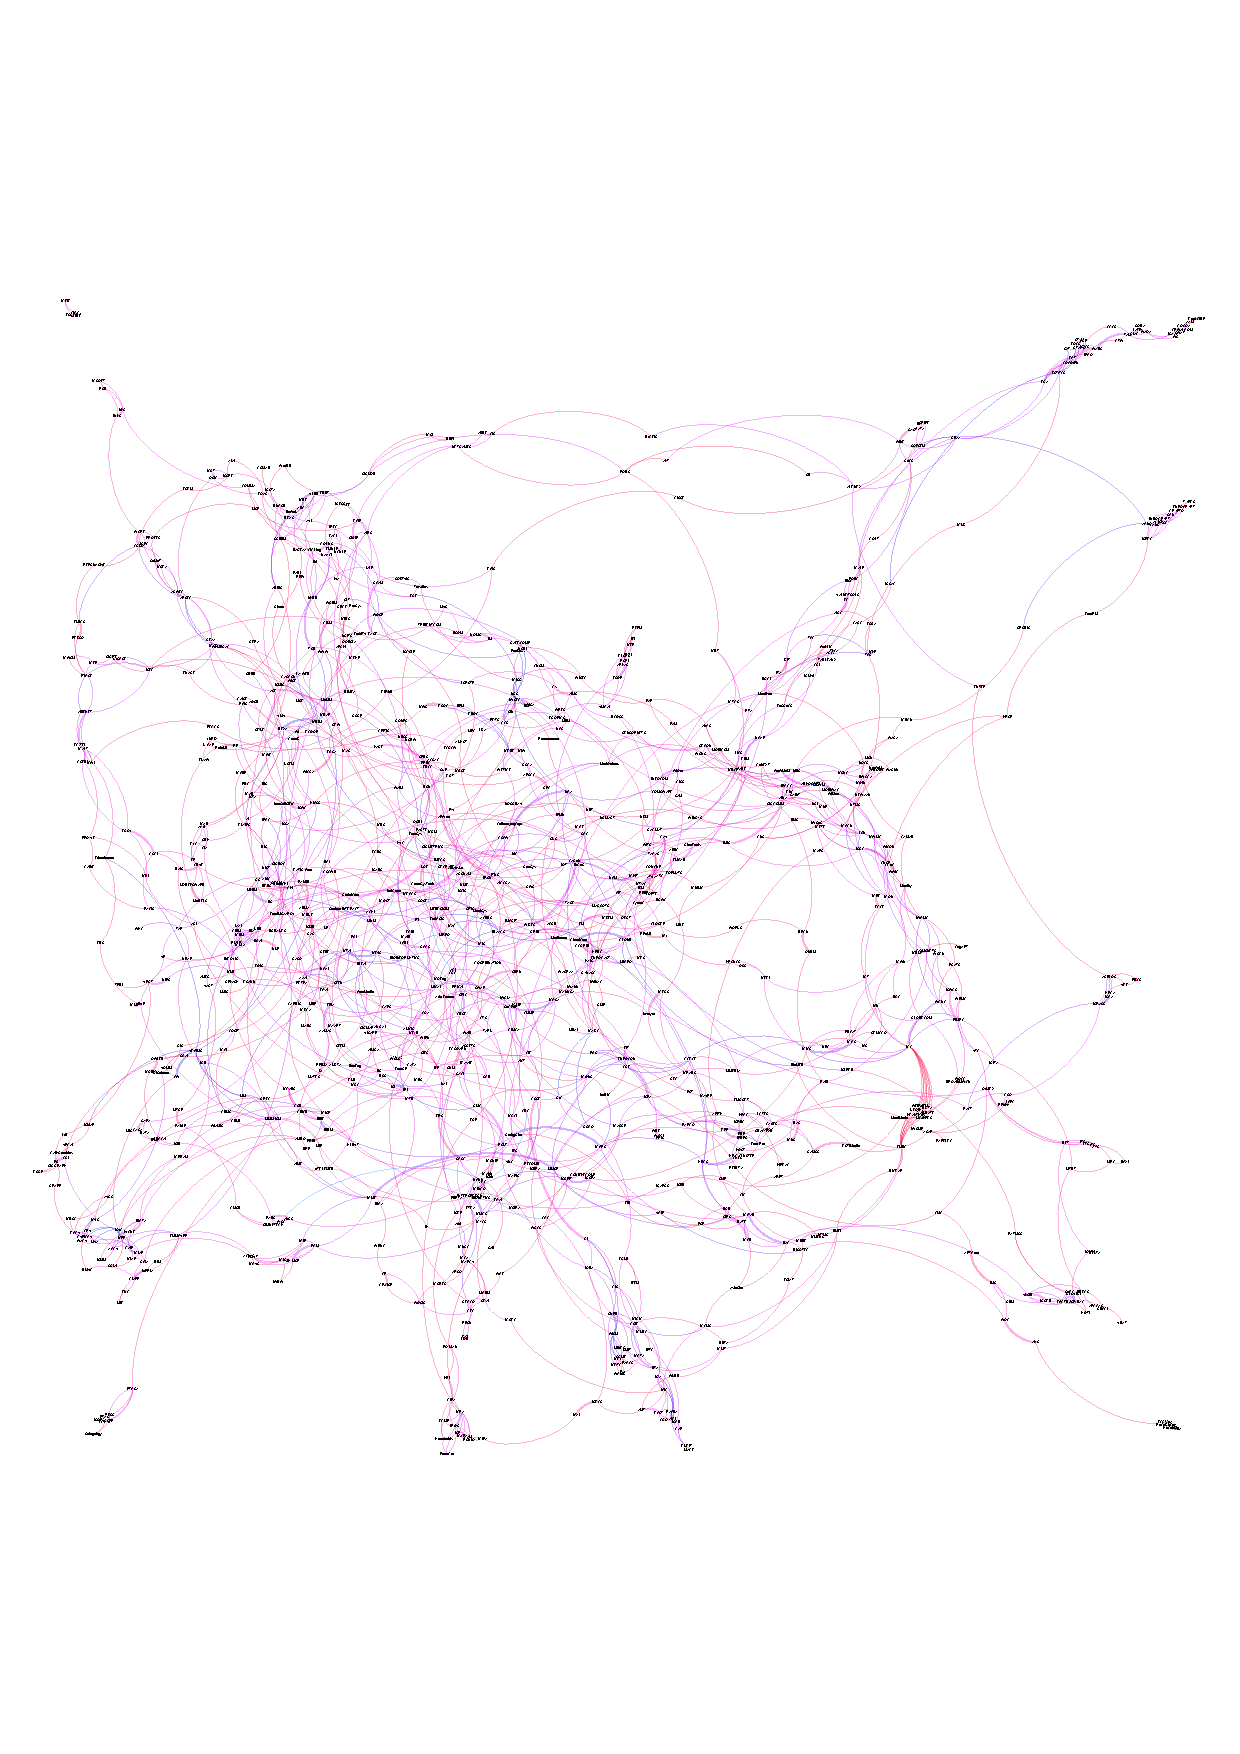
\includegraphics[width=0.7\linewidth]{chap3/gephi1.pdf}
\caption{可视化全景}
\label{fig:gephi1}
\end{figure}

如果我们把镜头拉近,可以看到节点之间的关系,脉络清晰可见,而且相关度的展示也很符合实际情况.
\begin{figure}
\centering
\includegraphics[width=0.7\linewidth]{../figures/chap3/gephi2}
\caption{可视化细节}
\label{fig:gephi2}
\end{figure}

图\ref{fig:gephi2}展示了具体的细节,选择放大的区域是以MOBICOM,INFOCOM等顶级会议为首的一系列网络,移动互联网相关会议.很显然,研究这些方向的研究者,对于这些学术会议应该都是比较熟悉的.而在阅读了其中一个学术会议论文后,那么我们也很自然地可以认为他对周围这几个会议中发表的学术论文会更有兴趣.

那么我们的推荐系统就可以围绕这一点来进行.一下就能想到的做法是按照论文所属会议,锁定距离比较接近的一些会议后,再来根据文章向量进行限定区域的论文推荐.这当然是一种合理的做法,但是还不够好,因为同样的会议中,也是包含了很多的方向的论文的.那么这些论文的方向,本身可能会根据不同的学术会议,会有少许的区别,这也是我们之前提到的会议本身对论文方向的影响.那我们要如何从这文章中剔除掉这里的影响呢?

看起来似乎很难,因为我们一直做的都是利用文章去构建会议,反过来怎么做就很让人发愁了.所幸,我们用于构建学术会议向量的方法,是去取文章向量的平均值.当时我们利用了聚类生成文章时词聚类频分布表示,可以进行向量加减的性质.那么同样的,我们何不反过来,从文章向量里减掉会议向量,不就很好的去掉了会议的影响了吗?

实际上,推荐系统也确实是按照这个思路实现的.我们在根据会议向量找到候选会议之后,再分别的求出其中每篇文章的相对向量

\begin{equation}
	\textbf{V}_{\mbox{relative}} = \textbf{V}_{\mbox{paper}} - \textbf{V}_{\mbox{conference}}
\end{equation}

然后再来根据这个相对向量来进行推荐.到这里,我们就完成了整个系统.推荐系统的参考代码片段如下

\begin{python}
# From recomm.py

def _vec_dis(a, b):
	assert len(a) == len(b) != 0, "Dimension Error in _vec_dis"  
	A, B = map(lambda e: math.sqrt(sum(map(lambda c:c*c, e))), [a,b])
	A_B = sum(map(lambda c: c[0] * c[1], zip(a,b)))
	try:
		res = A_B / (A * B)
	except ZeroDivisionError:
    	return 0.0
	return res

def recommend(cur_paper_id, k):
	cur_doc_vec = look_up_doc_vec(cur_paper_id)
	cur_confer = paper2confer[cur_paper_id]	
	confers = get_confer_neighbor(cur_confer)	
	relative_doc_vecs = gen_relative_doc_vec(confers)
	vec_dis = lambda a: _vec_dis(gen_relative_doc_vec(cur_paper_id), a)
	k_recomms = sorted(
		key=lambda c:c[1],
		map(vec_dis, relative_doc_vecs),
		reverse=True	
		)[:k]
	return map(lambda c:c[0], k_recomms)
	
\end{python}


